\documentclass[12pt,a4paper,headsepline,bibliography=totoc,listof=totoc,headinclude=false,footinclude=false,BCOR5mm]{scrreprt} % use larger type; default would be 10pt

%\usepackage[latin1]{inputenc} % set input encoding (not needed with XeLaTeX)
\usepackage[utf8x]{inputenc}
\usepackage{color}
\usepackage{hyperref}
\usepackage{url}
\usepackage{eurosym}
\usepackage{appendix}
\usepackage{listings}

\usepackage{subfig}
\usepackage{tikz}
\usepackage{mcode}


\usepackage{filecontents}

%%% PACKAGES
\usepackage{a4,booktabs}
\usepackage[ngerman]{babel}
\usepackage[lmargin=2.5cm, rmargin=1.5cm]{geometry}
\usepackage{amsmath,amssymb}
%\usepackage{fancyhdr}

\usepackage{array} % for better arrays (eg matrices) in maths
\usepackage{paralist} % very flexible & customisable lists (eg. enumerate/itemize, etc.)
\usepackage{verbatim} % adds environment for commenting out blocks of text & for better verbatim
\usepackage{subfig} % make it possible to include more than one captioned figure/table in a single float
\usepackage{graphicx}


 \usepackage[tc]{titlepic}
\usetikzlibrary{matrix}

% These packages are all incorporated in the memoir class to one degree or another...

%%% HEADERS & FOOTERS
%\usepackage{fancyhdr} % This should be set AFTER setting up the page geometry

\usepackage{scrpage2}
\pagestyle{scrheadings}
\clearscrheadfoot
\automark[section]{chapter}
\ihead[]{\leftmark}
\ohead[]{\rightmark}
\ofoot[\pagemark]{\pagemark}


\setlength{\topmargin}{-0.5in}
\setlength{\textheight}{9.5in}

\makeatletter 
\renewcommand*\bib@heading{\addchap{\bibname}\@mkboth{\bibname}{}


} 
\makeatother

\setkomafont{pagehead}
{\normalfont\sffamily\mdseries}
%\renewcommand{\headrulewidth}{0pt} % customise the layout...
%\fancyhf{} %alle Kopf- und Fußzeilenfelder bereinigen
%\fancyhead[L]{\title} %Kopfzeile links
%\fancyhead[C]{} %zentrierte Kopfzeile
%\fancyhead[R]{Name} %Kopfzeile rechts
%\renewcommand{\headrulewidth}{0.4pt} %obere Trennlinie
%\fancyfoot[C]{\thepage} %Seitennummer
%\renewcommand{\footrulewidth}{0.4pt} %untere Trennlinie

%\fancyhead[OR]{} % "O" steht für "odd", also ungerade Seiten
%\fancyhead[ER]{} % "E" für "even", also gerade Seiten.


%%% SECTION TITLE APPEARANCE
\usepackage{sectsty}
\allsectionsfont{\sffamily\mdseries\upshape} % (See the fntguide.pdf for font help)
% (This matches ConTeXt defaults)

%%% ToC (table of contents) APPEARANCE
%\usepackage[nottoc,notlof,notlot]{tocbibind} % Put the bibliography in the ToC
\usepackage[titles,subfigure]{tocloft} % Alter the style of the Table of Contents
\renewcommand{\cftsecfont}{\rmfamily\mdseries\upshape}
\renewcommand{\cftsecpagefont}{\rmfamily\mdseries\upshape} % No bold!
\renewcommand{\chapterheadstartvskip}{\vspace*{-2\topskip}}
%%% END Article customizations

%%% The "real" document content comes below...

\DeclareMathOperator*{\argmax}{arg\!\,max}

\begin{document}
\begin{titlepage}
\thispagestyle{empty}
 \begin{center}
 \begin{figure}[htbp]
    \centering
    \subfloat{
\includegraphics[width=0.4\textwidth]{feulogo}}\hspace{7.5em}
     \subfloat{
\includegraphics[width=0.375\textwidth]{wiwilogo}}\\
 \centering
  \vspace*{1.0cm}
    \subfloat{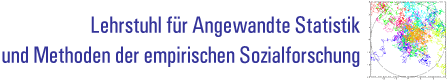
\includegraphics[width=0.75\textwidth]{rechtsfoto}}
\end{figure}

   


  %\vspace*{1.5cm}

  \vspace*{2.5cm}
 {\bf \Large Zustandsraummodelle und Kalman-Filter}
 \vspace*{3.5cm} \\
 {\Large Seminararbeit\\von\\}
 \vspace{0.5cm}
 {\large \bfseries Corvin Idler\\}
c/o European External Action Service, Delegation Australia, Diplomatic Pouch, \\1049 Brussels, BELGIUM\\
 +61 41 471 288, idler@uni-koblenz.de
 \vfill



\begin{table}[h]
	\centering
	\begin{tabular}{|l| l|}\hline
		Studiengang & Bachelor Wirtschaftsinformatik\\ \hline
		Betreuer & Dipl.-Kffr. Marina Lorenz\\ \hline
		Matrikelnummer & 7529953\\ \hline
		Arbeit vorgelegt am: & 13.04.2012\\ \hline
	\end{tabular}
\end{table}

 \end{center}
\end{titlepage}
\tableofcontents


 
\chapter{Einleitung}\label{einl}

Die vorliegende Arbeit hat den nach seinem Erfinder Rudolf E. K\'alm\'an benannten Kalman-Filter\cite{Kalman1960,Kalman1961} zum Inhalt. In seiner Urform handelt es sich dabei um eine rekursive Berechnungsvorschrift der Methode der kleinsten Quadrate\footnote{least squares algorithm}\cite{Legendre1805,Gauss1809} im Kontext der messwertbasierten Sch\"atzung linearer dynamischer endlichdimensionaler stochastischer Systeme in Zustandsraumdarstellung.
Seinen Durchbruch in der Praxis erfuhr der Filter durch Verwendung einer weiterentwickelten Version\footnote{extende Kalman-Filter} im Rahmen der Mondlandung der Apollo 11 Mission\cite{Schmidt1985}. Eine interessante historische Abhandlung \"uber seine Rolle in der Raumfahrt von Stanley F. Schmidt, dem die erste erfolgreiche Computerimplementierung des Algorithmus zugerechnet wird, findet sich in \cite{Schmidt1985}. Es ist anzumerken, dass der Filter schon vor  R. K\'alm\'an in nahezu identischer Form durch Peter Swerling ver{\"o}ffentlicht wurde  \cite{Swerling1958,Swerling1959}, der daf{\"u}r jedoch nie wirklich die ihm geb{\"u}hrende wissenschaftliche Anerkennung erhielt. Der Kalman-Filter geh\"ort heute zum Standardrepertoire der Praktiker vieler wissenschaftlicher Disziplinen und ist seit langem nicht mehr nur auf die Aeronautik als sein Ursprungsanwendungsgebiet beschr{\"a}nkt. So lassen sich viele praktische Problemstellungen durch eine Menge interessierender m{\"o}glicherweise stochastischer Gr\"o{\ss}en beschreiben, deren zeitliche Entwicklung durch Differential-\footnote{im zeitkontinuierlichen Fall} bzw. Differenzengleichungen\footnote{im zeitdiskreten Fall} modelliert wird. Im Paradigma der sogenannten Zustandsraumdarstellung wird dabei die jeweils vorliegende Problemstellung als ein dynamisches System verstanden, dessen zeitliche Entwicklung sich aus den oben genannten systembeschreibenden Differential- bzw. Differenzengleichungen ableiten l\"asst und dessen intrinsischer Zustand zu jedem Zeitpunkt durch eine Menge sogenannter Zustandsvariablen repr\"asentiert wird. Diese Gr\"o{\ss}en sind jedoch per definitionem unbekannt, oft stochastischer Natur und lassen sich nur \"uber m\"oglicherweise verrauschte Messungen sch\"atzen. Die Problematik kann man sich exemplarisch anhand der Umfeldbeobachtung, wie in Abb. \ref{beob} illustriert, veranschaulichen. \begin{figure}[h!]
    \centering
    \includegraphics[width=0.80\textwidth]{estimator}
\caption{Das Zustandssch\"atzproblem im Kontext der Umfeldbeobachtung. \\ Entnommen aus \cite[S. 72]{OReilly1996TLM} }\label{beob}
\end{figure}
Die beiden Kernkomponenten stellen die Umgebung (The World) und derjenige, der die Umgebung beobachtet und  eine Beschreibung von ihr erlangen m\"ochte (The Estimator) dar. Die Zust\"ande (hidden states) der externen Welt sind nicht direkt erfassbar oder bekannt, es kann nur auf Basis der Sensordaten, die ein Zustand hervorruft, auf selbigen zur\"uckgeschlossen werden. 
Bei der Beobachtung einer Umgebung ist also immer mindestens ein Sensor involviert, der durch eine bestimmte Funktion (mapping function) die Umweltzust\"ande auf Sensor- oder Messdaten 
abbildet.  Diese Funktion bezeichnet man auch als Sensor-, Mess- oder Beobachtungsmodell. Um nun R\"uckschl\"usse auf den Zustand der beobachteten Umgebung ziehen zu k\"onnen, braucht man neben dem Sensormodell auch ein Modell der Umgebung. Dieses abstrahiert 
bzw. reduziert die Umgebung auf eine Menge von interessierenden Gr\"o{\ss}en und modelliert 
deren zeitliche Entwicklung. Hat man sowohl ein Systemmodell als auch ein Sensormodell aufgestellt, dann kann man versuchen, auf Basis beider Modelle und unter Verwendung der Sensordaten den Zustand des 
Systems zu bestimmen (inverse mapping), um somit eine abstrakte Beschreibung der 
aktuellen Umgebung zu erlangen. In ganz \"ahnlicher Weise lassen sich eine Vielzahl von Problemstellungen wie beispielsweise radarbasierte Objektverfolgung\footnote{tracking} oder auch {\"o}konometrische Fragestellungen als ein Sch\"atzproblem unbekannter Zust\"ande eines dynamischen Systems verstehen. Dem Kalman-Filter-Algorithmus kommt dabei die Aufgabe zu, in m{\"o}glichst optimaler Art und Weise das inverse mapping vorzunehmen, also das Sch{\"a}tzen der Systemzust{\"a}nde auf Basis der Messdaten sowie des System- und Messmodells \cite{Anderson1992}.

Der Aufbau der weiteren Ausf{\"u}hrungen dieser Arbeit gestaltet sich wie folgt: In Kapitel \ref{gl} erfolgt eine mathematische Beschreibung der Problemstellung und des Filters. In Kapitel \ref{aw} wird dann an einem praktischen Anwendungsbeispiel aus der \"Okonometrie die Arbeitsweise des Kalman-Filter zur Parametersch{\"a}tzung im Kontext der Zinsstrukturmodellierung vorgeführt.

\chapter{Grundlagen}\label{gl}
\section{Ausgangsproblemstellung}\label{problem}


Von dem konkreten Beispiel der Umfeldbeobachtung aus Kapitel \ref{einl} abstrahiert, ist das Ausgangsproblem nochmal in Abbildung \ref{sysabst} schematisch visualisiert.
\begin{figure}[h!]
    \centering
    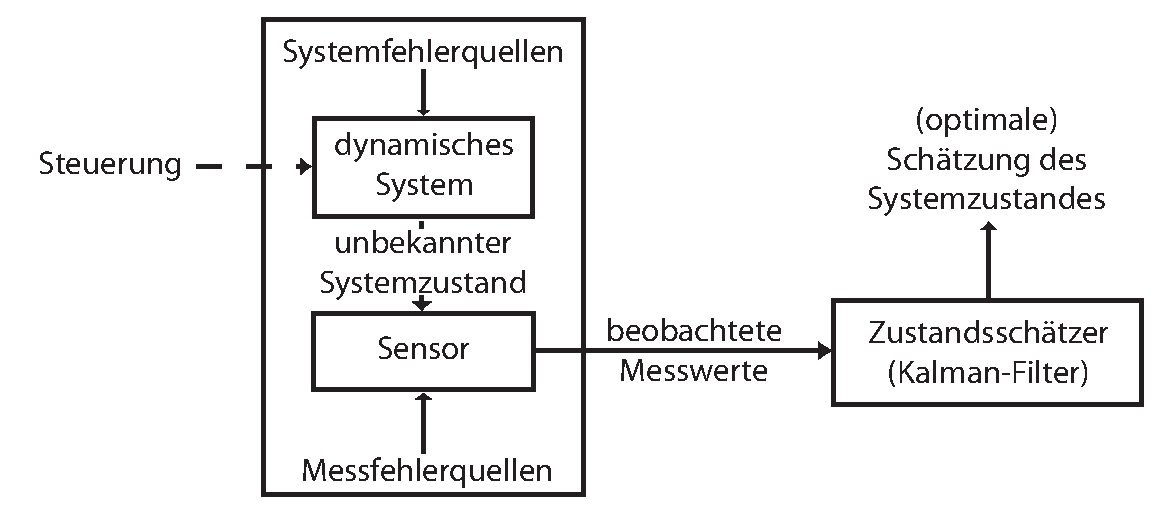
\includegraphics[width=0.90\textwidth]{system}
\caption{Schema des typischen Einsatzkontexts eines Kalman-Filters. \\In Anlehnung an \cite[S. 5]{Maybeck79} }\label{sysabst}
\end{figure} Es gilt die Zust{\"a}nde eines linearen stochastischen dynamischen Systems auf Basis verrauschter Beobachtungswerte m{\"o}glichst optimal zu sch{\"a}tzen. Hierzu muss man, wie schon in Kapitel \ref{einl} erw{\"a}hnt, ein System- und ein Messmodell aufstellen und zus{\"a}tzlich eine Rechenvorschrift zum Zustandssch{\"a}tzen formulieren. Dies wird in mathematischer Form im folgenden Abschnitt beschrieben.


\section{Mathematische Beschreibung}\label{math}
Die folgenden Ausf\"uhrungen beschr\"anken sich aus Platzgr\"unden auf die zeitdiskrete Version des Kalman-Filters. 
\subsection{Systemmodell}
Das System- bzw. Zustandsmodell sei im Allgemeinen \cite[S. 10]{Sorenson1970}\cite[S. 38ff]{Kalman1960} durch folgendes lineares rekursives Gleichungssystem ausgedr\"uckt
\begin{equation}\label{systemequc} \begin{split} & \underbrace{x_{t+1}}_{\text{Zustandsvektor}} = \underbrace{\Phi_{t+1}}_{\text{\"Ubergangsmatrix}} \cdot \underbrace{x_{t}}_{\text{Zustandsvektor}}+\underbrace{\Xi_{t+1}}_{\text{Steuermatrix}}\cdot\underbrace{u_{t}}_{\substack{\text{exogener} \\ \text{ Steuervektor}}}+\underbrace{w_{t}}_{\text{Rauschgr\"o{\ss}e}};  \\&  x_t \in \mathbb{R}^{n}, \Phi_t \in \mathbb{R}^{n \times n}, u_t \in \mathbb{R}^{l}, \Xi_t \in \mathbb{R}^{n \times l}, w_t \sim N(0,Q_t), Q_t \in \mathbb{R}^{n \times n}, \forall t \in \mathbb{N}_{0}
\end{split} \end{equation}
Dabei ist der n-dimensionale Zustandsvektor $x_{t+1}$ zum Zeitpunkt $t+1$ eine durch die Übergangs\-matrix $\Phi_{t+1}$ festgelegte Linearkombination des Zustandsvektors des vorherigen Zeitpunktes, dem zus{\"a}tzlich ein wei{\ss}er Rauschvektor\footnote{Prozess- bzw. Systemrauschen} $w_t$ mit Kovarianzmatrix $Q_t$ additiv {\"u}berlagert wird. In manchen F\"allen ist in der Systemmodellierung zus{\"a}tzlich noch die M{\"o}glichkeit eines exogenen Kontrollinputs {\"u}ber die Steuermatrix $\Xi_{t+1}$ und den Inputvektor $u_t$ vorgesehen. Sofern in der vorliegenden Problemauspr{\"a}gung kein externer Kontrollinput vorgesehen ist, entf{\"a}llt dieser Term, sodass sich Gleichung \ref{systemequc} vereinfacht zu:
 \begin{equation}\label{systemequ} \begin{split} & \underbrace{x_{t+1}}_{\text{Zustandsvektor}} = \underbrace{\Phi_{t+1}}_{\text{\"Ubergangsmatrix}} \cdot \underbrace{x_{t}}_{\text{Zustandsvektor}}+\underbrace{w_{t}}_{\text{Rauschgr\"o{\ss}e}};  \\&  x_t \in \mathbb{R}^{n}, \Phi_t \in \mathbb{R}^{n \times n}, w_t \sim N(0,Q_t), Q_t \in \mathbb{R}^{n \times n}, \forall t \in \mathbb{N}_{0}
\end{split} \end{equation}
Wenn man sich vergegenw{\"a}rtigt, dass $\Phi_t$ und  $Q_t$ zwar mathematisch zeitvariant modelliert werden k{\"o}nnen,  in der Praxis aber eine solche Modellierung bzw. Kalibrierung meist alles andere als trivial ist, weil man daf{\"u}r ja eine sehr genaue Kenntnis der System- und Rauschdynamik haben m{\"u}sste, so wird schnell klar, dass diese beiden Matrizen meist als zeitinvariant angenommen werden. Gleichung \ref{systemequ} lautet dann:
 \begin{equation}\label{systemequf} \begin{split} & x_{t+1} = \Phi  x_{t} + w_{t};  \\&  x_t \in \mathbb{R}^{n}, \Phi \in \mathbb{R}^{n \times n}, w_t \sim N(0,Q), Q \in \mathbb{R}^{n \times n}, \forall t \in \mathbb{N}_{0}
\end{split} \end{equation}

\subsection{Messmodell}
Das Beobachtungs- bzw. Messmodell ist in Anlehnung an \cite[S. 10]{Sorenson1970} durch folgendes Gleichungssystem gegeben:
 \begin{equation}\label{messequ} \begin{split} & \underbrace{z_{t}}_{\text{Messvektor}} = \underbrace{H_{t}}_{\text{Sensormatrix}} \cdot \underbrace{x_{t}}_{\text{Zustandsvektor}}+\underbrace{v_{t}}_{\text{Rauschgr\"o{\ss}e}};  \\& z_t \in \mathbb{R}^{m},  x_t \in \mathbb{R}^{n}, H_t \in \mathbb{R}^{n \times m}, v_t \sim N(0,R_t), R_t \in \mathbb{R}^{n \times n}, \forall t \in \mathbb{N}_{0}
\end{split} \end{equation}
Auch hierbei gilt, dass die Sensormatrix $H_{t}$ und die Rauschkovarianzmatrix $R_t$ in der Praxis meist als zeitinvariant angenommen werden, weil sonst die genaue zeitliche Dynamik des Sensors und seines Rauschens bekannt sein m{\"u}sste. Daraus ergibt sich folgendes vereinfachte Sensormodell:
 \begin{equation}\label{messequf} \begin{split} & z_{t} = H_{t} x_{t} + v_{t};  \\& z_t \in \mathbb{R}^{m},  x_t \in \mathbb{R}^{n}, H \in \mathbb{R}^{n \times m}, v_t \sim N(0,R), R \in \mathbb{R}^{n \times n}, \forall t \in \mathbb{N}_{0}
\end{split} \end{equation}
\section{Zustandssch{\"a}tzung}
Die zu l{\"o}sende Aufgabe, welche in Kapitel \ref{problem} bereits nicht-mathematisch veranschaulicht wurde, besteht nun darin, in rekursiver Weise zuk{\"u}nftige Zust{\"a}nde $x_{t+1}$  auf Basis des vergangenen gesch{\"a}tzten Zustandes $\hat{x}_t$ in Form von $\hat{x}_{t+1}$ so zu sch{\"a}tzen, dass die dabei auftretenden Diskrepanzen mit den Messwerten $z_t$ im Sinne der Methode der kleinsten Quadrate minimal werden, also eine Minimierung der Sch{\"a}tzfehlervarianzen vorgenommen wird \cite{Anderson1992}. Da dies, wie sp{\"a}ter noch zu sehen ist, ein sich periodisch wiederholender zweigeteilter Vorgang ist, gebietet es sich f{\"u}r die weiteren Ausf{\"u}hrungen in der Notation zu reflektieren, ob man sich auf den Zeitpunkt vor Eintreffen eines Messwertes (a priori) oder nach Eintreffen zus{\"a}tzlicher Information in Form eines Messwertes (a posteriori) bezieht \cite[S.2]{Welch2006}. In der Literatur (z.B. \cite{Sorenson1970}) wird dies oft durch tiefgestellte Zeitindizes der Form $t / t$ gel{\"o}st, von denen sich der erste Index auf den Betrachtungszeitpunk bezieht und der zweite Index auf den Zeitpunkt, von dem das zur Verf{\"u}gung stehende Wissen stammt. Parallelen zur Bayesschen Sch{\"a}tztheorie sind hier offensichtlich und nicht rein zuf{\"a}llig, wie im letzten Teil dieses Kapitels aufgezeigt wird. 

Zustandssch{\"a}tzungen erfolgen in der Regel in zwei Schritten: 1) Vorhersage des n{\"a}chsten Zustandes und 2) Korrektur der Sch{\"a}tzung auf Basis neu eingetroffener Messdaten. In Schritt 1) trifft man eine Vorhersage {\"u}ber den aktuellen Systemzustand in folgender Form:
 \begin{equation}\label{predict} \underbrace{\hat{x}_{t/t-1}}_{\substack{\text{a priori Sch{\"a}tzung} \\ \text{aktueller Zeitschritt}}} = \Phi  \underbrace{\hat{x}_{t-1/t-1}}_{\substack{\text{a posteriori Sch{\"a}tzung}\\ \text{vorheriger Zeitschritt}}}
 \end{equation}
Interessant wird es nun im zweiten Schritt bei der Frage, wie man bei Eintreffen neuer Messwerte eine m{\"o}glichst optimale Sch{\"a}tzung des Zustandes aus einer Kombination der alten Sch{\"a}tzung und der neu eingetroffenen Messwerte vornehmen kann. Mathematisch l{\"a}sst sich die wie folgt formulieren \cite{Sorenson1970}:
 \begin{equation}\label{update} \underbrace{\hat{x}_{t/t}}_{\substack{\text{a posteriori Sch{\"a}tzung}\\ \text{aktueller Zeitschritt}}} = \overbrace{\Phi  \underbrace{\hat{x}_{t-1/t-1}}_{\substack{\text{a posteriori Sch{\"a}tzung}\\ \text{vorheriger Zeitschritt}}}}^{\text{Zeitinnovation}= \hat{x}_{t/t-1}}+ K_t \overbrace{\left(\overbrace{\underbrace{z_t}_{\substack{\text{Messwert}\\ \text{aktueller Zeitschritt}}}}^{\text{reale Messwerte}} - \overbrace{H \underbrace{\hat{x}_{t/t-1}}_{\substack{\text{a priori Sch{\"a}tzung}\\ \text{aktueller Zeitschritt}}}}^{\text{Messwertvorhersage =}\hat{z}_t}\right)}^{\text{Messinnovation = Vorhersagefehler}}
 \end{equation}
Die a posteriori Sch{\"a}tzung wird also dargestellt als Linearkombination der a priori Sch{\"a}tzung und der Diskrepanz zwischen hypothetischen Messwerten, basierend auf der a priori Sch{\"a}tzung und den neu eingetroffenen wirklichen Messwerten. Man kombiniert also die Sch{\"a}tzung des Zustandes, in den sich das System in der Zwischenzeit laut Systemmodell hinbewegt haben m{\"u}sste (Zeitinnovation), mit der Diskrepanz zwischen dem, was man in diesem Fall h{\"a}tte messen m{\"u}ssen und dem, was man f{\"u}r den aktuellen Zeitpunkt wirklich gemessen hat (Messinnovation). Die sogenannte Gain- oder Kalman-Matrix $K_t \in \mathbb{R}^{n \times m} $ ist dabei offensichtlich von zentraler Bedeutung. Die Spezifizierung einer optimalen Wahl f{\"u}r $K_t$ ist einer der wissenschaftlichen Verdienste von R. Kalman.  Optimal heißt in diesem Zusammenhang, dass der a posteriori Sch{\"a}tzfehler zwischen dem wahren und dem geschätzten Zustand $e_{t/t} = x_t -  \hat{x}_{t/t}$ minimiert werden soll. Von Interesse sind dabei die  a posteriori Fehlerkovarianzmatrix  $P_{t/t}$ mit dem Erwartungswert \begin{equation}\label{aposteriorifehler} P_{t/t}=\text{E}[e_{t/t} e_{t/t}^T]\Leftrightarrow \text{cov}(x_t -  \hat{x}_{t/t})  \end{equation}
  und die a priori Fehlerkovarianzmatrix $P_{t/t-1}$ mit dem a priori Sch{\"a}tzfehler $e_{t/t-1} = x_t -  \hat{x}_{t/t-1}$ und dem Erwartungswert  \begin{equation} \label{apriorifehler} P_{t/t-1}=\text{E}[e_{t/t-1} e_{t/t-1}^T]\Leftrightarrow \text{cov}(x_t -  \hat{x}_{t/t-1}) \end{equation} Setzt man Gleichung (\ref{messequ}) f{\"u}r $z_{t}$ in Gleichung (\ref{update}) ein, wendet Gleichung (\ref{predict}) auf den ersten Summanden in Gleichung (\ref{update}) an und setzt den dadurch resultierenden Term f{\"u}r $\hat{x}_{t/t}$ in Gleichung (\ref{aposteriorifehler}) ein so erh{\"a}lt man
\begin{equation}\label{herleitung} P_{t/t}=\text{cov}\left(x_t - \left( \hat{x}_{t/t-1} + K_{t}\left(H x_{t} +v_{t} - H  \hat{x}_{t/t-1} \right)\right)\right)  \end{equation}
Diese Gleichung l{\"a}sst sich unter Verwendung matrix-algebraischer Rechenregeln \cite[S. 10]{Sorenson1970}\cite[S. 39ff.]{Kalman1960}\cite[S. 3]{Welch2006}  weiterentwickeln zu: 
 \begin{equation}\label{herl}\begin{split}
& P_{t/t}=\text{cov}\left(x_t - \left( \hat{x}_{t/t-1} + K_{t}\left(H x_{t} +v_{t} - H  \hat{x}_{t/t-1} \right)\right)\right)\\
\Leftrightarrow & P_{t/t}=\text{cov}\left(\left(I - K_{t}H\right)\left(x_t - \hat{x}_{t/t-1}\right)\right)+ \text{cov}\left(K_{t}v_{t}\right)\\
\Leftrightarrow & P_{t/t}=\left(I - K_{t}H\right)\text{cov}\left(x_t - \hat{x}_{t/t-1}\right)\left(I - K_{t}H\right)^{T}+ K_{t}\text{cov}\left(v_{t}\right)K_{t}^{T}\\
\end{split} \end{equation} 
Durch Anwendung von Gleichung (\ref{apriorifehler}) erh{\"a}lt man schlussendlich folgende sogenannte Joseph-Form\footnote{benannt nach Peter. D. Joseph} \cite[S. 136]{Mohinder2008}:
\begin{equation}\label{joseph} P_{t/t}=\left(I - K_{t}H\right) P_{t/t-1} \left(I - K_{t}H\right)^{T}+ K_{t} R K_{t}^{T} \end{equation}
Es l{\"a}sst sich zeigen, dass die Minimierung des Erwartungswertes der mittleren quadratischen Abweichung  des a posteriori Sch{\"a}tzfehlers $e_{t/t} = x_t -  \hat{x}_{t/t}$ von der optimalen Wahl von $K_t$ abh{\"a}ngt  \cite[S. 10]{Sorenson1970}\cite[S. 39ff.]{Kalman1960}\cite[S. 3]{Welch2006}. Unter Bezug auf Gleichung (\ref{joseph}) gilt es dabei die Spur der Matrix  $P_{t/t}$ zu minimieren. Durch ausmultiplizieren der Terme in Gleichung (\ref{joseph}) und Bildung der Spur durch $\text{tr( )}$ erh{\"a}lt man: 
\begin{equation}\label{josephaus} \text{tr}(P_{t/t})=\text{tr}(P_{t/t-1} - K_{t}HP_{t/t-1}  - P_{t/t-1}  K_{t}^{T}H^{T} + K_{t}(H P_{t/t-1}  H^{T} + R)K_{t}^{T})\end{equation}
Um diese Spur in Bezug auf die Wahl von $K_{t}$ zu minimieren, wird die Matrixfunktion partiell nach $K_{t}$ abgeleitet und gleich Null gesetzt. Es ergibt sich somit mittels der Ableitungsgesetze f{\"u}r Matrixfunktionen und der Rechenregeln bez{\"u}glich der Spurbildung von Matrizen folgender Zusammenhang:
\begin{equation}\label{josephaussp} \frac{\partial \text{tr}(P_{t/t})}{\partial K_{t}}=-2(HP_{t/t-1})^{T} + 2K_{t}(H P_{t/t-1}  H^{T} + R)=0\end{equation}
Nach $K_{t}$ aufgel{\"o}st folgt dann als optimale Wahl f{\"u}r $K_{t}$:
\begin{equation}\label{gainmatrix} K_{t}=P_{t/t-1}H^T(\underbrace{HP_{t/t-1}H^T + R}_{\text{Residualkovarianz}})^{-1}
\end{equation} mit 
\begin{equation}\label{errorcovmatrix2} P_{t/t}= P_{t/t-1} -K_tH P_{t/t-1}
\end{equation} und 
\begin{equation}\label{errorcovmatrix} P_{t/t-1}=\Phi P_{t-1/t-1} \Phi^T + Q
\end{equation}
Die Gleichungen \ref{update} und \ref{gainmatrix}-\ref{errorcovmatrix} bezeichnet man in aller Regel als den Kalman-Filter. Interessant an Gleichung \ref{gainmatrix} ist, dass f{\"u}r eine gegen Null strebende Messfehlerkovarianzmatrix $R$, $K_t$ gegen $H^{-1}$ strebt und somit die Messinnovation gegen{\"u}ber der Zeitinnovation {\"u}bergewichtet wird. Umgekehrt gilt, dass wenn die a priori Fehlerkovarianzmatrix $P_{t/t-1}$ gegen Null strebt, $K_t$ ebenfalls gegen Null strebt und somit die Messinnovation gegen{\"u}ber der Zeitinnovation untergewichtet wird. Der Filter passt sich also sozusagen automatisch in seinem Gewichtungsverhalten an, je nachdem wie (un)zuverl{\"a}ssig seine vorherigen Sch{\"a}tzungen waren und je nachdem wie (un)zuverl{\"a}ssig das Sensorverhalten ist. Der Filter besitzt also einen eingebauten R{\"u}ckkopplungssteuermechanismus.

\subsection{Kalman-Filter-Algorithmus}
Der Kalman-Filter in seiner Form als mathematisches Gleichungssystem kann in eine praktische Rechenvorschrift als zweigeteilter rekursiv-zyklischer Algorithmus umgewandelt werden. Mit jedem Zeitschritt wird ein neuer Rekursionsschritt  des Algorithmus vorgenommen. Wie in Abbildung \ref{kalman} ersichtlich, wird in dem Zeit-Innovationsschritt eine a priori Vorhersage (Pr{\"a}diktion) f{\"u}r den Systemzustand und die Fehlerkovarianzmatrix vorgenommen. In dem darauf folgenden Mess-Innovationsschritt wird nach Eintreffen neuer Messdaten eine a posteriori beobachtungsbasierte Bestimmung des Kalman-Gain sowie eine Korrektur der Zustands- und Fehlerkovarianzsch{\"a}tzung vorgenommen.

\begin{figure}[h!]
    \centering
    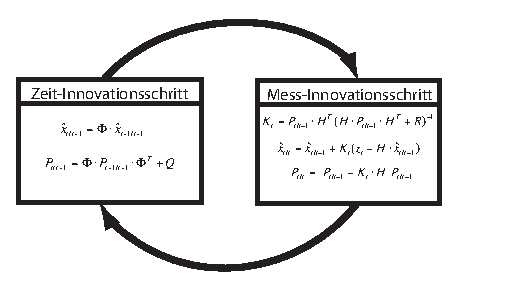
\includegraphics[width=0.80\textwidth]{kalman}
\caption{Ablaufschema des Kalman-Filter-Algorithmus \\In Anlehnung an \cite[S. 24]{Welch2006} }\label{kalman}
\end{figure}

\subsection{Bezug zur Bayesschen Sch{\"a}tztheorie}
Der Kalman-Filter kann auch im Paradigma der Bayesschen Sch{\"a}tztheorie betrachtet werden und als Gau{\ss}scher Bayes-Filter zur Zustandssch{\"a}tzung von Markovprozessen verstanden werden, wie im Folgenden aufgezeigt wird. Die Ausf{\"u}hrungen basieren dabei auf \cite{Idler2005}. 
Die zu sch{\"a}tzende Wahrscheinlichkeitsdichte besteht aus
\begin{displaymath}p\left(x_{t}\mid z_{1}, \ldots, z_{t}\right),\end{displaymath} wobei $z_{1}, \ldots, z_{t}$ die Sequenz aller bisherigen Sensordaten, ausgehend vom Zeitpunkt $1$ bis zum aktuellen Zeitpunkt $t$, repr{\"a}sentiere. Unter Anwendung der bayesschen Regel, l{\"a}sst sich dieser Term ausdr{\"u}cken durch

\begin{equation}\label{bayesformula}
p\left(x_{t}\mid z_{1}, \ldots, z_{t}\right)=\frac{p\left(z_{t}\mid x_{t}, z_{1}, \ldots, z_{t-1}\right)p\left(x_{t}\mid z_{1}, \ldots, z_{t-1}\right)}{p\left(z_{t}\mid z_{1}, \ldots, z_{t-1}\right)}.
\end{equation} Durch die f{\"u}r den zu beschreibenden Prozess angenommene Markov-Umgebung erster Ordnung  kann (\ref{bayesformula}) umgeformt werden zu

\begin{equation}\label{bayesplusmarkov}
p\left(x_{t}\mid z_{1}, \ldots, z_{t}\right) =\frac{p\left(z_{t}\mid x_{t}\right)p\left(x_{t}\mid z_{1}, \ldots, z_{t-1}\right)}{p\left( z_{t}\mid z_{1}, \ldots, z_{t-1}\right)}.
\end{equation} und durch Anwendung des Satzes der totalen Wahrscheinlichkeit kann (\ref{bayesplusmarkov}) in die eine rekursive Berechnung erm{\"o}glichende Gleichung

\begin{equation}\label{secondmarkov}
p\left(x_{t}\mid z_{1}, \ldots, z_{t}\right)=\frac{p\left(z_{t}\mid x_{t}\right)}{p\left(z_{t}\mid z_{1}, \ldots, z_{t-1}\right) }\int p\left(x_{t}\mid x_{t-1}\right)p\left(x_{t-1}\mid z_{1}, \ldots, z_{t-1}\right)\mathrm{d} x_{t-1}
\end{equation} {\"u}berf{\"u}hrt werden. Sei mit $\eta_{t}$ folgende in Abh{\"a}ngigkeit zum Sensormodell stehende Normalisierungskonstante bezeichnet \cite[S. 175]{Arulampalam2002ATO},

\begin{equation}
\eta_{t}^{-1}=p\left(z_{t}\mid z_{1}, \ldots, z_{t-1}\right)=\int p\left(z_{t}\mid x_{t}\right)p\left(x_{t}\mid z_{1}, \ldots, z_{t-1}\right)\mathrm{d}x_{t},
\end{equation} 

kann (\ref{secondmarkov}) umgeformt werden zu

\begin{equation}\label{equ:bayesfilter}
p\left(x_{t}\mid z_{1}, \ldots, z_{t}\right)=\eta_{t} \underbrace{p\left(z_{t}\mid x_{t}\right)}_{\text{Sensormodell}}\int \underbrace{p\left(x_{t}\mid  x_{t-1}\right)}_{\text{Systemmodell}}p\left(x_{t-1}\mid z_{1}, \ldots, z_{t-1}\right)\mathrm{d} x_{t-1}.
\end{equation} Dies ist die im Allgemeinen als \textbf{Bayesfilter} bezeichnete Gleichung zur rekursiven Absch{\"a}tzung des aktuellen Systemzustandes, basierend auf allen bisherigen Messdaten, in Form einer bedingten Wahrscheinlichkeitsdichte {\"u}ber dem Zustandsraum. Der Bezug zum Kalman-Filter wird klar, wenn man sich verdeutlicht, dass eine algorithmische Realisierung der Bayesfiltergleichung (\ref{equ:bayesfilter})  in der Regel ebenfalls in zwei Schritten abl{\"a}uft:

\begin{enumerate}
\item Vorhersage: $p\left(x_{t}\mid z_{1}, \ldots, z_{t-1}\right)=\int p\left( x_{t} \mid  x_{t-1}\right)p\left(x_{t-1}\mid z_{1}, \ldots, z_{t-1}\right)\mathrm{d}x_{t-1}$
\item Aktualisierung: $p\left(x_{t}\mid z_{1}, \ldots, z_{t}\right)=\eta_{t} p\left(z_{t}\mid x_{t}\right)p\left(x_{t}\mid z_{1}, \ldots, z_{t-1}\right)$
\end{enumerate} In einem Pr{\"a}diktionsschritt (Vorhersage) wird das Systemmodell verwendet, um basierend auf der sogenannten Chapman-Kolmogorov-Gleichung (\ref{equ:chapman}) eine Voraussage dar{\"u}ber zu treffen, in welchem Zustand sich das System im n{\"a}chsten Zeitschritt vermutlich befinden wird. Unter der erw{\"a}hnten Chapman-Kolmogorov-Gleichung versteht man dabei folgende Integralgleichung
\begin{equation}\label{equ:chapman}
p\left(x_{t}\mid z_{1}, \ldots, z_{t-1}\right)=\int p\left(x_{t} \mid x_{t-1}\right)p\left(x_{t-1}\mid z_{1}, \ldots, z_{t-1}\right)\mathrm{d}x_{t-1},
\end{equation}
die auf Basis des Systemmodells die \textbf{a posteriori}  Wahrscheinlichkeitsdichte \\$p\left(x_{t-1}\mid z_{1}, \ldots, z_{t-1}\right)$ aus dem Zeitschritt $t-1$ in eine Randverteilung {\"u}berf{\"u}hrt, welche gleich der \textbf{a priori} Wahrscheinlichkeitsdichte $p\left(x_{t}\mid z_{1}, \ldots, z_{t-1}\right)$ zum Zeitpunkt $t$ ist. Die Gleichung entspricht somit genau dem Integralterm des Bayesfilters aus (\ref{equ:bayesfilter}).
 Der Term \begin{math}p\left(x_{t}\mid x_{t-1}\right)\end{math} repr{\"a}sentiert das System- bzw. Prozessmodell \cite[S. 35]{Schmitt2004VPS}. Beim Eintreffen neuer Sensordaten wird im zweiten Schritt des Bayesfilters (Aktualisierung) auf Basis der pr{\"a}diktierten a priori Wahrscheinlichkeitsdichte $p\left(x_{t}\mid z_{1}, \ldots, z_{t-1}\right)$ zum Zeitpunkt $t$,  die a posteriori Wahrscheinlichkeit $p\left(x_{t}\mid z_{1}, \ldots, z_{t}\right)$ zum Zeitpunkt $t$ durch folgende Gleichung bestimmt
\begin{equation}p\left(x_{t}\mid z_{1}, \ldots, z_{t}\right)=\eta_{t} p\left(z_{t}\mid x_{t}\right)p\left(x_{t}\mid z_{1}, \ldots, z_{t-1}\right). \end{equation} Der Term $p\left(z_{t}\mid x_{t}\right)$ modelliert das Sensor- bzw. Beobachtungsmodell und wird als Beobachtungswahrscheinlichkeit bezeichnet. Die Interpretation des Kalman-Filters als Gau{\ss}scher Bayesfilter l{\"a}sst sich pr{\"a}gnant nochmal durch folgendes Gleichungssystem aufzeigen:

 \begin{equation}\label{kalmbay}\begin{split}
p\left(x_{t}\mid x_{t-1}\right) & \sim N(\Phi x_{t-1},Q) \\
p\left(z_{t}\mid x_{t}\right) & \sim N(H x_{t},R) \\
p\left(x_{t-1}\mid z_{1}, \ldots, z_{t-1}\right) & \sim N(\hat{x}_{t-1/t-1},P_{t-1/t-1}) \\
\end{split} \end{equation} 

\section{Likelihoodfunktion im Kalman-Filter Kontext}
Im Hinblick auf den im n{\"a}chsten Kapitel folgenden praktischen Teil der Arbeit wird in diesem Abschnitt kurz darauf eingegangen, wie eine Likelihoodfunktion als Beiprodukt aus den in dem Kalmanfilter berechneten Matrizen definiert werden kann. Von besonderem Interesse daf{\"u}r sind die Messinnovation, die im Folgenden mit $\zeta_t$ bezeichnet sei und die Residualkovarianzmatrix, welche durch $\Sigma_t$ symbolisiert sei:
 \begin{equation}\label{like1}\begin{split}
\zeta_t & = z_t - H\hat{x}_{t/t-1} \\
\Sigma_t  &=  HP_{t/t-1}H^T + R
\end{split} \end{equation} 
Mit Hilfe dieser beiden Terme l{\"a}sst sich nach \cite[S. 34ff]{Bolder2001} und \cite[S. 9ff]{Duffee2004} folgende Likelihoodfunktion aufstellen \cite[S. 83ff.]{Mazzoni2007}.:
 \begin{equation}\label{like2}
\Lambda_t = \Lambda _{t-1} - n \log (2 \pi ) 2^{-1}- \frac{1}{2} \left(\log \left|\Sigma_t\right| +\zeta_{t}^{T}\Sigma_{t}^{-1}\zeta_{t}\right) 
 \end{equation} und daraus ein aggregierter Likelihoodwert f{\"u}r den Zeitraum $t = 1$ bis $T$ ableiten durch:
 \begin{equation}\label{like3}
\Lambda _T = \sum_{t=1}^{T} \Lambda _t 
 \end{equation}
Wie in Kapitel \ref{paramscha} noch gezeigt wird, spielt diese Likelihoodfunktion eine bedeutende Rolle, wenn man neben den Systemzust{\"a}nden auch noch eventuelle Modellparameter absch\"atzen muss bzw. von verschiedenen zur Auswahl stehenden Modellen das am besten geeignete aussuchen muss.


\chapter{{\"O}konometrisches Anwendungsbeispiel}\label{aw}
Im Folgenden wird der Einsatz des Kalmanfilters im Kontext der Parameterbestimmung ausgew{\"a}hlter affiner Zinsstrukturmodelle vorgestellt \cite{Duffie1996,Cox1985,Vasicek1977}. Die Ausf{\"u}hrungen basieren {\"u}berwiegend auf \cite{Bolder2001,Idler2011}. Es werden fundierte Kenntnisse der allgemeinen Problematik der Zinsstrukturmodellierung vorausgesetzt und aus Platzgr{\"u}nden auf eine Einf{\"u}hrung in das Problemfeld an dieser Stelle verzichtet und stattdessen auf die einschl{\"a}gige Literatur \cite{Damiano2007,Rudolf2000,Wilmott2007,Andersen2010b,Andersen2010a,Hughston2003,Rebonato2003} und \cite{Idler2011} verwiesen. 

\section{Datenbasis}\label{datenbasis} Als Datenbasis f{\"u}r die folgenden Betrachtungen wird auf historische LIBOR-Geld\-markt\-zinsdaten\footnote{London Interbank Offered Rate; Berechnung: \url{ http://www.bbalibor.com/bbalibor-explained/the-basics}} zur{\"u}ckgegriffen, welche t{\"a}glich von der British Bankers' Association (BBA)\footnote{Pinners Hall, 105-108 Old Broad Street, London EC2N 1EX, United Kingdom} ver{\"o}ffentlicht werden und im Internet-Archiv\footnote{\url{http://web.archive.org/web/20090413091623/http://www.bba.org.uk/bba/jsp/polopoly.jsp?d=141&a=627
}} abrufbar sind. Die Untersuchungen in dieser Arbeit wurden auf den Zeitraum 2000 bis 2008  und die Laufzeiten 1-12 Monate eingeschr{\"a}nkt. \begin{figure}[h!]
    \centering
\subfloat{\label{liboralla}\includegraphics[width=0.45\textwidth]{plainliborone2twelvemonth00208a.eps}}
\subfloat{\label{liborallb}\includegraphics[width=0.45\textwidth]{plainliborone2twelvemonth00208b.eps}}
\caption[gegl{\"a}ttete Zinsstruktur \euro-LIBOR 2000-2008, Tageswerte, 1-12 Monate Laufzeit]{gegl{\"a}ttete Zinsstruktur \euro-LIBOR 2000-2008, Tageswerte, 1-12 Monate Laufzeit} \label{libor}
\end{figure} Bei den LIBOR-Zinsdaten aus  Abbildung \ref{libor} handelt es sich um j{\"a}hrliche Zinss{\"a}tze f{\"u}r feste diskrete Laufzeiten $\tau$. Symobilisieren $L(\tau); \tau \in \frac{1}{12}, ..., \frac{12}{12}$ die diskreten LIBOR-S{\"a}tze f{\"u}r die Laufzeiten $\tau$ von einem bis 12 Monaten\footnote{ausgedr{\"u}ckt in Jahresbruchteilen}, dann k{\"o}nnen daraus implizierte Kurse $P(\tau)$ f{\"u}r hypothetische ausfallsrisikofreie Nullkuponanleihen mit korrespondierenden Laufzeiten wie folgt berechnet werden \cite[S. 16ff.]{Chance2004}:

\begin{equation}\label{liborbond}
P(\tau) = \left( 1+L(\tau)\tau \right)^{-1}; \forall \tau \in \frac{1}{12}, ... , \frac{12}{12}
\end{equation}
F{\"u}r obige Berechnung sei ein Jahr, in {\"U}bereinstimmung mit der LIBOR-Berechnungs\-konvention\footnote{\url{http://www.bbalibor.com/technical-aspects/calculating-interest}}, auf 360 Tage normiert. Ein Monat sei f{\"u}r die Zwecke dieser Arbeit aus Vereinfachungsgr{\"u}nden auf 30 Tage normiert. 
Die Berechnungsergebnisse aus Gleichung (\ref{liborbond}) stellen die Zinsstruktur in Form von Diskontfaktoren dar. Aus ihnen lassen sich die laufzeitabh{\"a}ngigen Kassazinsraten\footnote{(continously compounded) spot rates} $z(\tau)$ wie folgt berechnen:
\begin{equation}\label{kassa}
z(\tau) =  - \frac{\ln P(\tau)}{\tau} =  \frac{\ln ( 1 + L(\tau)\tau)}{\tau} 
 \end{equation}
Die instantane Kassazinsrate\footnote{short rate} $r(t)$ zum Zeitpunkt $t$ l{\"a}sst sich aus $z(\tau)$ durch Grenzwertbildung ableiten:
\begin{equation}\label{short}
r(t) =  \lim_{\tau \to 0} z(\tau) =   \lim_{\tau \to 0} - \frac{\ln P(\tau)}{\tau}
 \end{equation}
In dem Paradigma der affinen Zinsstrukturmodelle wird ihr zeitlicher Verlauf im Einfaktorfall durch folgende stochastische Differentialgleichung beschrieben:
\begin{equation}\label{shortprocess}
dr(t) = \underbrace{A_{0}dt}_{\text{Drift}} + \underbrace{A_{1}dW(t)}_{\text{Diffusion}}
 \end{equation}
Zwei popul{\"a}re Auspr{\"a}gungen dieser Modellklasse  \cite[S. 16]{Bolder2001}, welche den short-rate-Prozess als Ornstein-Uhlenbeck-Prozess modellieren, bestehen in dem Zinsstrukturmodell nach \cite{Vasicek1977} mit 
\begin{equation}\label{vasi}\begin{split}
& A_{0} = \kappa (\bar{\theta} - r(t)) ; \\ & A_{1} = \sigma; \\ & \bar{\theta}=\theta - \frac{\sigma\lambda}{\kappa}
 \end{split} \end{equation}
und dem nach \cite{Cox1985} mit
\begin{equation}\label{cox}\begin{split}
& A_{0} = \kappa (\bar{\theta} - r(t)) ; \\ & A_{1} = \sigma\sqrt{r(t)}; \\ & \bar{\theta}=\theta - \frac{\sigma\lambda}{\kappa}
\end{split} \end{equation} Dabei bezeichnet $\theta$ einen langfristigen mittleren Zinssatz, $\kappa$ den Mittelwertr{\"u}ckkehrparameter, $\sigma$ die Volatilit{\"a}t und $\lambda$ den Marktpreis des Risikos der ungewissen zuk{\"u}nftigen Zinsentwicklung.

\section{Zinsstrukturmodell}
\subsection{Ein-Faktor-Fall}

Dem hier betrachteten Paradigma der affinen Zinsstrukturmodelle nach \cite{Duffie1996} liegt die Annahme zu Grunde, dass die Nullkuponanleihenpreisfunktion eine lineare Funktion der ihr zugrunde liegenden Zustandsvariablen ist, welche die Unsicherheit bzgl. der zuk{\"u}nftigen Zinsentwicklung bzw. -dynamik repr{\"a}sentiert \cite[S. 4]{Bolder2001}. Die Preisfunktion wird dabei allgemein wie folgt ausgedr{\"u}ckt: \begin{equation}\label{affin}
P(\tau) = e^{A(\tau)-B(\tau)r}
 \end{equation} Bei $A(t)$ und $B(t)$ muss es sich dabei um Funktionen handeln, die (wenn {\"u}berhaupt) nur deterministisch von der Zeit abh{\"a}ngen. Bei dem Vasicek-Modell \cite{Vasicek1977} ergeben sich diese Funktionen laut Herleitung in \cite[S. 16ff]{Bolder2001} aus Gleichung \ref{vasi} wie folgt:
\begin{equation}\label{affinvasi}\begin{split}
 B(\tau) &= \frac{1}{\kappa} (1- e^{-\kappa\tau}); \\  A(\tau) & = \frac{\gamma(B(\tau)-\tau)}{\kappa^2} - \frac{\sigma^2B^2(\tau)}{4\kappa}; \\  \gamma & =\kappa^2\left(\theta - \frac{\sigma\lambda}{\kappa}\right) - \frac{\sigma^2}{2}
\end{split} \end{equation}
F{\"u}r das CIR-Modell nach \cite{Cox1985} ergibt sich laut \cite[S. 42ff]{Bolder2001} unter Verwendung von Gleichung \ref{cox} folgender Zusammenhang:
\begin{equation}\label{affinCIR}\begin{split}
 B(\tau) & = \frac{2(e^{\gamma r}-1)}{(\gamma + \kappa + \lambda)(e^{\gamma r}-1)+2\gamma};\\ A(\tau) & =\ln\left(\frac{2\gamma e^{\frac{(\gamma + \kappa + \lambda)r}{2}} }{(\gamma + \kappa + \lambda)(e^{\gamma r}-1)+2\gamma} \right)^{\frac{2\kappa\theta}{\sigma^{2}}}; \\  \gamma & =\sqrt{(\kappa + \lambda)^{2}+2\sigma^{2}}
\end{split} \end{equation}

\subsection{Multi-Faktor-Fall}
Erweitert man die klassischen Einfaktorans{\"a}tze von \cite{Vasicek1977} und \cite{Cox1985} um weitere Faktoren, welche derselben Modellierung folgen, so kann man die instantane Short-Rate $r$ als eine Linearkombination von $n$ m{\"o}glicherweise korrelierter Zustandsvariablen $x_{1}, ... , x_{n}$ modellieren. Konkret wird in \cite[S. 18ff]{Bolder2001} f{\"u}r das Vasicek Modell folgender Mehrfaktorzusammenhang vorgestellt
\begin{equation}\label{affinvasim}\begin{split}
P(\tau) & = e^{A(\tau)-\sum^{n}_{j=1}B_{j}(\tau)x_{j}} \\
 B_{j}(\tau) &= \frac{1}{\kappa_{j}} (1- e^{-\kappa_{j}\tau}); \\  A(\tau) & = \sum_{j=1}^{n} \frac{\gamma_{j}(B_{j}(\tau)-\tau)}{\kappa_{j}^2} - \frac{\sigma_{j}^2B_{j}^2(\tau)}{4\kappa_{j}} \\& + \sum_{i,j:i\neq j} \frac{\sigma_{ij}}{2\kappa_{i}\kappa_{j}}\left(\tau - B_{i}(\tau)-B_{j}(\tau) + \frac{1}{\kappa_{i}+\kappa_{j}}\left(1 - e^{-(\kappa_{i}+\kappa_{j})(r)}\right)\right); \\  \gamma_{j} & =\kappa_{j}^2\left(\theta_{j} - \frac{\sigma_{j}\lambda_{j}}{\kappa_{j}}\right) - \frac{\sigma_{j}^2}{2}
\end{split} \end{equation} und f{\"u}r das CIR Modell entsprechend:
\begin{equation}\label{affincir}\begin{split}
P(\tau) & = e^{\sum^{n}_{j=1}A_{j}(\tau)-B_{j}(\tau)x_{j}} \\
 B_{j}(\tau) & = \frac{2(e^{\gamma_{j} r}-1)}{(\gamma_{j} + \kappa_{j} + \lambda_{j})(e^{\gamma_{j} r}-1)+2\gamma_{j}};\\ A_{j}(\tau) & =\ln\left(\frac{2\gamma_{j} e^{\frac{(\gamma_{j} + \kappa_{j} + \lambda_{j})r}{2}} }{(\gamma_{j} + \kappa_{j} + \lambda_{j})(e^{\gamma_{j} r}-1)+2\gamma_{j}} \right)^{\frac{2\kappa_{j}\theta_{j}}{\sigma_{j}^{2}}}; \\  \gamma_{j} & =\sqrt{(\kappa_{j} + \lambda_{j})^{2}+2\sigma_{j}^{2}}
\end{split} \end{equation}
Ein exemplarisches mehrdimensionales Beobachtungs- und Systemmodell f{\"u}r das Vasicek Modell aus Gleichung (\ref{affinvasim}) l{\"a}sst sich laut \cite[S. 29ff]{Bolder2001} unter Annahme von 3 Zustandsvariablen ($x_t \in \mathbb{R}^{3}$) und einer Datenbasis von 12 unterschiedlichen Monatslaufzeiten $\tau_{1}, ..., \tau_{12}$ ($z_t \in \mathbb{R}^{12}$) wie folgt ableiten:
\begin{equation}
z_{t} = \left[ \begin{array}{c} -\frac{A(\tau_{1})}{\tau_{1}} \\ \vdots \\  -\frac{A(\tau_{{12}})}{\tau_{{12}}} \end{array} \right] +  \begin{bmatrix} &\frac{B_1(\tau_{1})}{\tau_{1}} & \frac{B_2(\tau_{1})}{\tau_{1}} & \frac{B_3(\tau_{1})}{\tau_{1}}\\ &\vdots & \vdots& \vdots \\ &\frac{B_1(\tau_{{12}})}{\tau_{{12}}} & \frac{B_2(\tau_{{12}})}{\tau_{{12}}} &  \frac{B_3(\tau_{{12}})}{\tau_{{12}}} \end{bmatrix}  x_t  +  v_t 
\end{equation}

\begin{equation}
  x_t   = \left[ \begin{array}{c} \theta_1(1-e^{-\kappa_{1}\Delta t}) \\\theta_2(1-e^{-\kappa_{2}\Delta t}) \\  \theta_3(1-e^{-\kappa_{3}\Delta t}) \end{array} \right] +  \begin{bmatrix} &e^{-\kappa_{1}\Delta t} & 0 & 0\\ &0 & e^{-\kappa_{2}\Delta t}&0  \\ &0 &0 &  e^{-\kappa_{3}\Delta t} \end{bmatrix}   x_{t-1}   +  w_t 
\end{equation}
Dabei kann das Messrauschen des Beobachtungsmodells konventionell in einer Diagonalmatrix $R$ modelliert werden, jedoch ergibt sich f{\"u}r das Systemrauschen folgender etwas komplexerer Zusammenhang:
\begin{equation}
w_t  \sim N(0,Q); Q =  \begin{bmatrix} &\frac{\sigma^{2}_{1}}{2\kappa_{1}} (1- e^{-2\kappa_{1}\Delta t}) & 0 & 0\\ &0 & \frac{\sigma^{2}_{2}}{2\kappa_{2}} (1- e^{-2\kappa_{2}\Delta t}) &0  \\ &0 &0 &\frac{\sigma^{2}_{3}}{2\kappa_{3}} (1- e^{-2\kappa_{3}\Delta t})  \end{bmatrix}   
\end{equation}
Analog kann man folgende Modelle f{\"u}r das CIR Modell aufstellen:


\begin{equation}
z_{t} = \left[ \begin{array}{c} \sum_{j=1}^{3}-\frac{A_j(\tau_{1})}{\tau_{1}} \\ \vdots \\ \sum_{j=1}^{3} -\frac{A_j(\tau_{{12}})}{\tau_{{12}}} \end{array} \right] +  \begin{bmatrix} &\frac{B_1(\tau_{1})}{\tau_{1}} & \frac{B_2(\tau_{1})}{\tau_{1}} & \frac{B_3(\tau_{1})}{\tau_{1}}\\ &\vdots & \vdots& \vdots \\ &\frac{B_1(\tau_{{12}})}{\tau_{{12}}} & \frac{B_2(\tau_{{12}})}{\tau_{{12}}} &  \frac{B_3(\tau_{{12}})}{\tau_{{12}}} \end{bmatrix} x_t  +  v_t 
\end{equation}
\begin{equation}
 x_t = \left[ \begin{array}{c} \theta_1(1-e^{-\kappa_{1}\Delta t}) \\\theta_2(1-e^{-\kappa_{2}\Delta t}) \\  \theta_3(1-e^{-\kappa_{3}\Delta t}) \end{array} \right] +  \begin{bmatrix} &e^{-\kappa_{1}\Delta t} & 0 & 0\\ &0 & e^{-\kappa_{2}\Delta t}&0  \\ &0 &0 &  e^{-\kappa_{3}\Delta t}  \end{bmatrix} x_{t-1}   +  w_t 
\end{equation}
Auch hier kann das Messrauschen des Beobachtungsmodells konventionell in einer Diagonalmatrix $R$ modelliert werden, das Systemrauschen ist jedoch bedeutend komplexer als im Vasicek Fall:
\begin{equation}
w_t  \sim N(0,Q); Q_{t} =  \begin{bmatrix} &\psi_{1} & 0 & 0\\ &0 & \psi_{2}  &0  \\ &0 &0 &\psi_{3} \end{bmatrix} x_{t-1} 
\end{equation}
mit 
\begin{equation}
\psi_{j} = \frac{\theta_{j}\sigma^{2}_{j}}{2\kappa_{j}}(1- e^{-\kappa_{j}\Delta t})^{2}+\frac{\sigma^{2}_{j}}{\kappa_{j}}(e^{-\kappa_{j}\Delta t}- e^{-2\kappa_{j}\Delta t})
\end{equation}

 \section{Parametersch{\"a}tzung}\label{paramscha}
In der im Anhang \ref{anhang} dargestellten praktischen Implementierung der bisher vorgestellten Konzepte, wird dem in Abschnitt \ref{datenbasis} beschriebenen LIBOR-Datensatz exemplarisch ein eindimensionales CIR-Modell durch Parametersch{\"a}tzung angepasst. Dabei wird der Kalman-Filter im Geiste des expectation–maximization (EM) Algorithmus \cite{Dempster1977} zur wiederholten rekursiven Berechnung der Likelihoodwerte f{\"u}r einzelne Parameterhypothesen herangezogen. Die eigentliche Optimierung der Parameterwerte wird in der dieser Arbeit zugrunde liegenden Implementierung (siehe S.\pageref{anhang}) durch Innere-Punkte-Verfahren (z.B. \cite{Waltz2006}) durchgef{\"u}hrt. Das Berechnungsergebnis nach erfolgreichem Durchlaufen des Algorithmus besteht im Idealfalle\footnote{je nach verwendetem Abbruchkriterium} aus einer maximum a posteriori (MAP) Sch{\"a}tzung der Parameterwerte f{\"u}r  $\theta, \kappa,  \sigma, \lambda$ bei der definitionsgem{\"a}ss der aggregierte Likelihoodwert $\Lambda _T$ aus Gleichung (\ref{like3}) maximal wird
\begin{equation}
\argmax_{\theta, \kappa,  \sigma, \lambda} \Lambda _T (\theta, \kappa,  \sigma, \lambda)
\end{equation}
F{\"u}r den vorliegenden Datensatz und die vorliegende Implementierung ergeben sich die folgende aus Tabelle \ref{MAPPara} ersichtliche maximum a posteriori Sch{\"a}tzung der Parameter.
\begin{table}[h!]
\begin{center}
  \begin{tabular}{ | l | l | l | l |l |l |}
    \hline
    $\theta$ & $\kappa$  & $\sigma$ &   $\lambda$ & $\Lambda _T$   \\ \hline
  0.0324  & 0.0981 & 0.0189 & -0.0903  & -1.627$*10^{5}$   \\ \hline
  
    \hline
    \end{tabular}\caption{MAP Parametersch{\"a}tzung f{\"u}r 1-Faktor-CIR-Modell, \euro-LIBOR 2000-2008, Tageswerte, 1-12 Monate Laufzeit}\label{MAPPara}
\end{center}     
\end{table}

Die Rauschmatrix des Beobachtungsmodelles wird in der vorliegenden Implementierung ebenfalls als Teil der zu sch{\"a}tzenden bzw. zu optimierenden Parameter modelliert. Als Sch{\"a}tzung ergibt sich untige $12 \times 12$ Diagonalmatrix
\begin{equation}
R =  \text{diag}\begin{bmatrix}0.24, 0.17, 0.12, 0.09, 0.05, 0.02, 0.00, 0.02, 0.05, 0.06, 0.08, 0.10
  \end{bmatrix} *10^{-2}
\end{equation}
Abschlie{\ss}end sei der Vollst{\"a}ndigkeit halber angemerkt, dass ein alternativer Ansatz zur Parametersch{\"a}tzung im Kontext des Kalmanfilters darin besteht, die zu sch{\"a}tzenden Parameter explizit in einem erweiterten Zustandsraum zu modellieren und durch den Kalman-Filter gemeinsam mit den {\"u}rspr{\"u}nglichen Zust{\"a}nden mitsch{\"a}tzen zu lassen \cite[S. 83ff.]{Mazzoni2007}. Auf diese Vorgehensweise soll jedoch nicht weiter eingegangen werden.

\interlinepenalty10000
\bibliographystyle{alphaurl}
\bibliography{biblio,da}
\renewcommand\thechapter{}
\appendix



%\appendixpage
%\addappheadtotoc
\chapter{Anhang}\label{anhang}
%http://www.mathworks.com/matlabcentral/fileexchange/27493-kalman-filter-application
\lstset{language=Matlab}

\lstinputlisting{TreasuryYieldKF.m}
\lstinputlisting{loglik.m}
\begin{titlepage}
\thispagestyle{empty}
Hiermit versichere ich an Eides statt, dass ich die Seminararbeit selbst{\"a}ndig und ohne Inanspruchnahme fremder Hilfe angefertigt habe. Ich habe dabei nur die angegebenen Quellen und Hilfsmittel verwendet und die aus diesen w{\"o}rtlich oder inhaltlich entnommenen Stellen als solche kenntlich gemacht. Die Arbeit hat in gleicher oder {\"a}hnlicher Form noch keiner anderen Pr{\"u}fungsbeh{\"o}rde vorgelegen. Ich erkl{\"a}re mich damit einverstanden, dass die Arbeit mit Hilfe eines Plagiatserkennungsdienstes auf enthaltene Plagiate {\"u}berpr{\"u}ft wird.

  \vspace*{2.5cm}

Datum: \hfill 
  \vspace*{1.5cm}

Ort: \hfill 
  \vspace*{1.5cm}

Unterschrift: \hfill

\end{titlepage}
\end{document}
